\part{Práctica 2}
\setcounter{section}{0}
\section{Ejercicio 1}
\begin{center}
    \parbox{12cm}{\justify\textit{Explica brevemente qué es un sistema de control de versiones distribuido y sus diferencias con respecto a uno centralizado. Entra en la web de Git y revisa la documentación. Busca manuales, tutoriales, etc. de Git. Describe y compara con Git algún otro sistema de control de versiones distribuido (Mercurial, etc.).
    }}
\end{center}

Un \textbf{sistema de control de versiones distribuido} es una forma de control de versiones en la cuál el código, incluyendo el histórico, está replicado en las computadoras de cada desarrollador \cite{wikipedia_2020:Distributed_Version_Control}. Esto permite a cada desarrollador trabajar en el código sin necesidad de estar conectado a un servidor central \cite{juancarlosfernandez_2010}.
Las ventajas que ofrece un sistema distribuido frente a uno centralizado son:
\begin{itemize}
    \item No hay una copia canónica.
    \item Soporta operaciones desconectadas: La mayoría de operaciones comunes como confirmaciones, consultas del historial, diff, y revertir cambios son rápidas, porque no se necesita conexión con el sistema central.
    \item Cada copia de trabajo es una copia de seguridad.
    \item Ramas experimentales: crear y eliminar ramas es rápido y simple.
    \item Fomenta la colaboración entre desarrolladores, permitiendo por ejemplo compartir cambios sin necesidad de confirmarlos en el servidor central.
\end{itemize}

\begin{figure}[H]
    \centering
    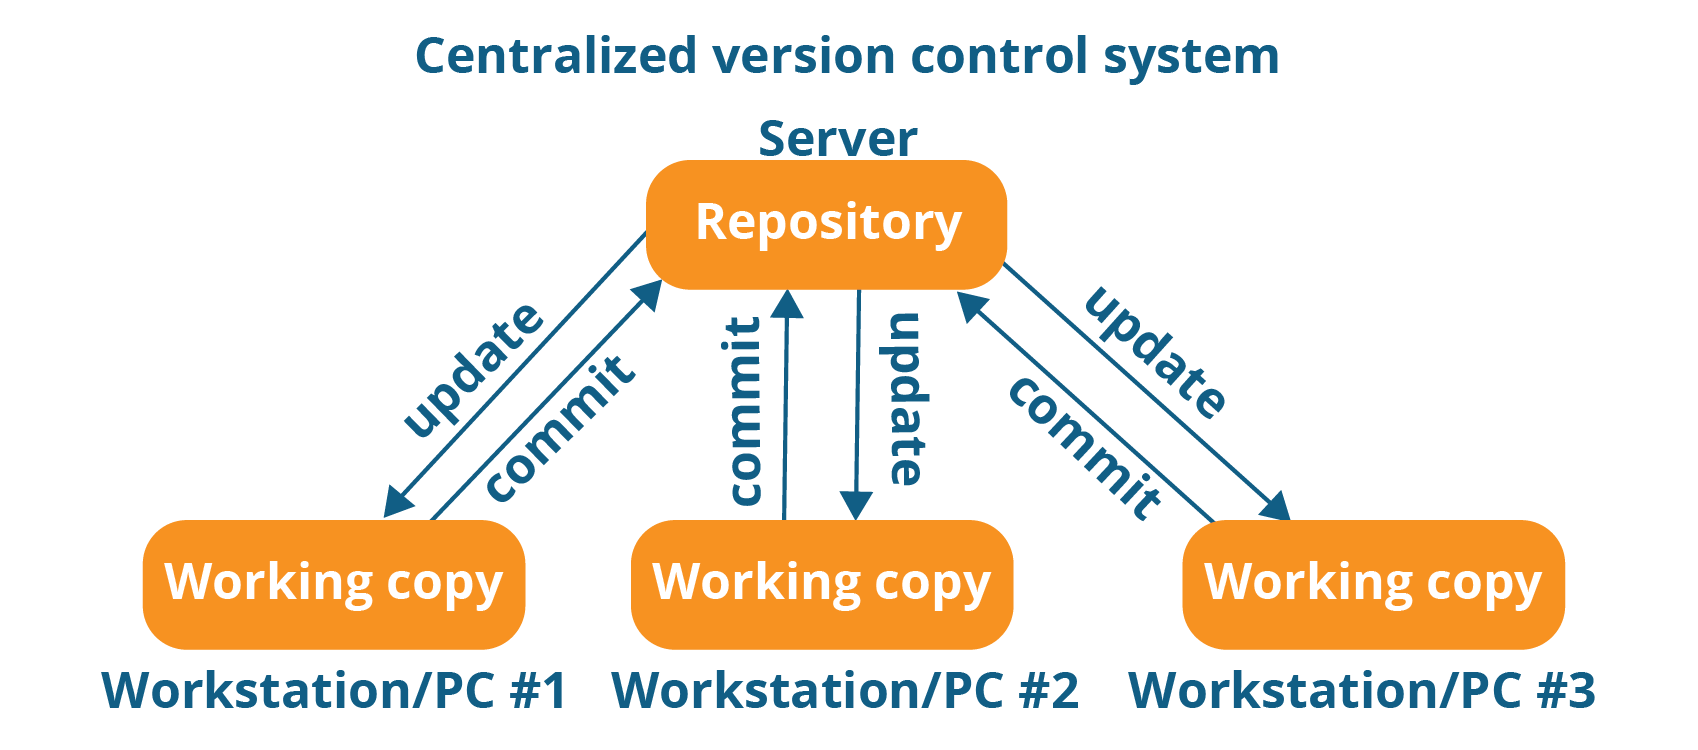
\includegraphics[scale=0.16]{sistema-centralizado}
    \caption{Esquema de control de versiones centralizado}
    \label{fig:sistema-centralizado}
\end{figure}


\begin{figure}[H]
    \centering
    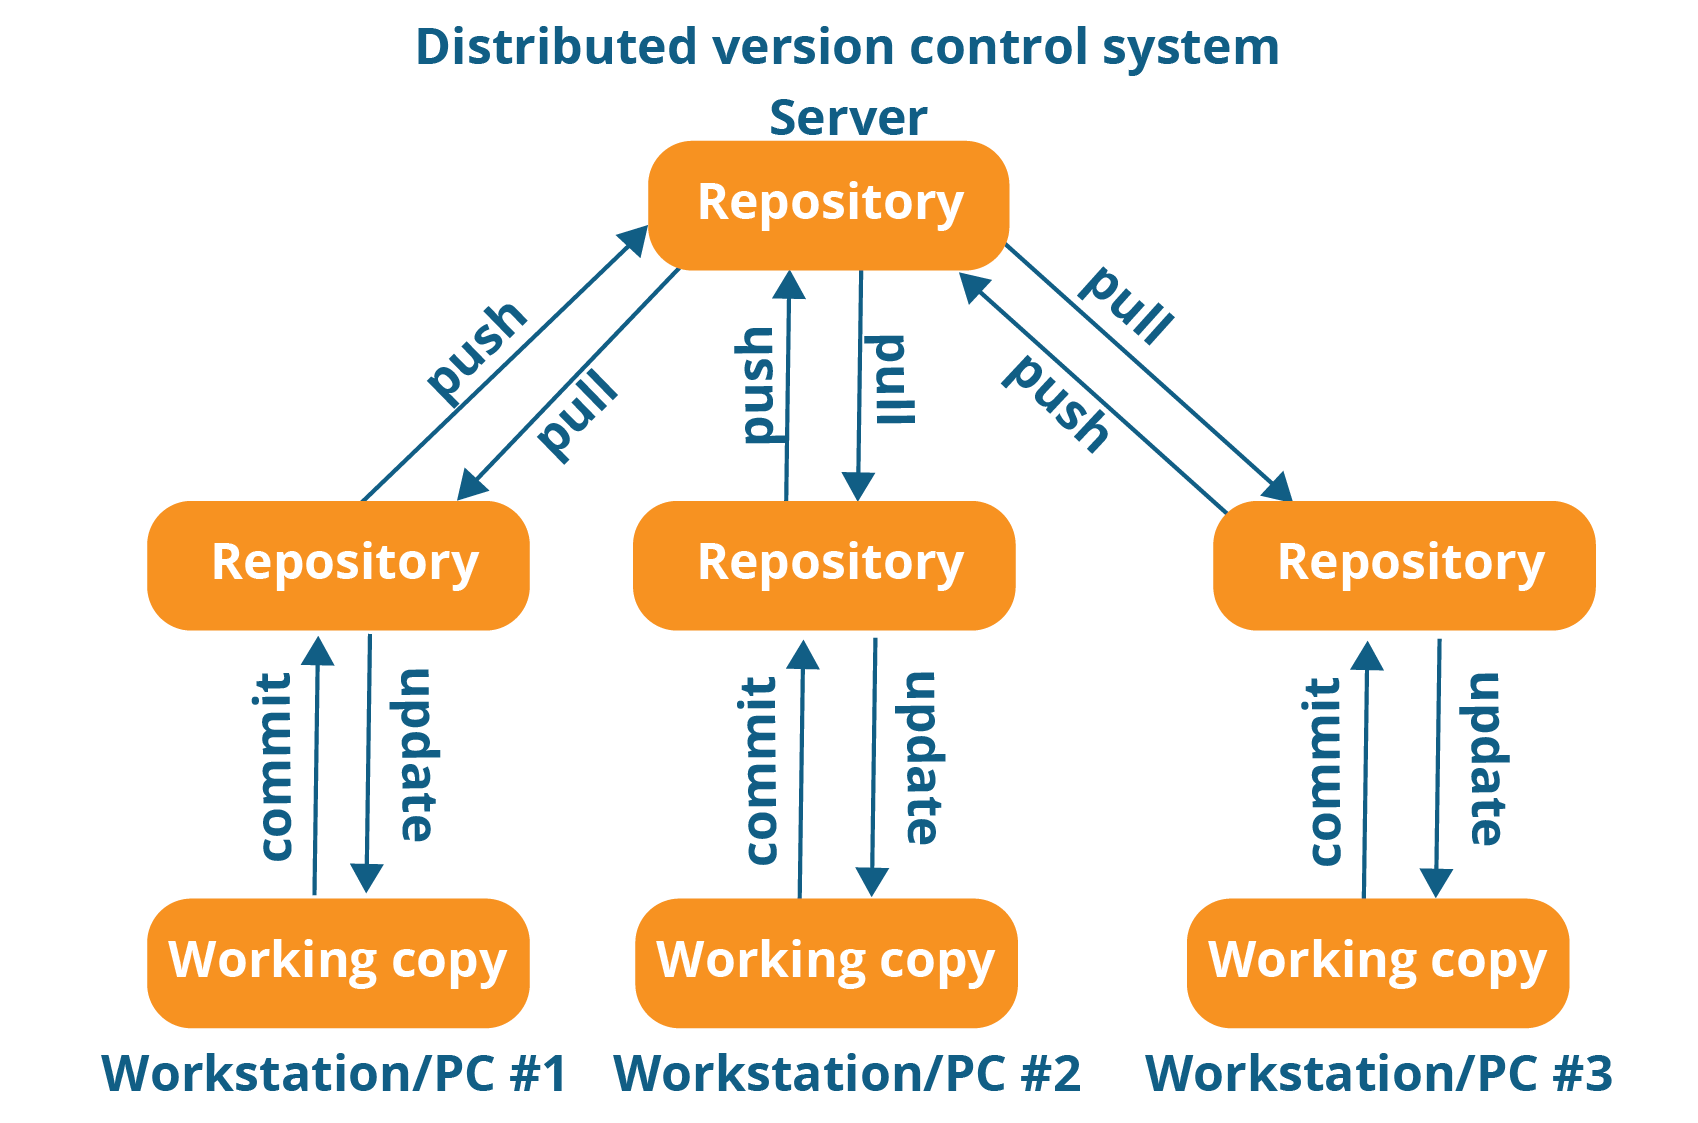
\includegraphics[scale=0.16]{sistema-distribuido}
    \caption{Esquema de control de versiones distribuido}
    \label{fig:sistema-distribuido}
\end{figure}


La web de Git tiene un apartado de \href{https://git-scm.com/doc}{documentación} con enlaces a los documentos siguientes:
\begin{itemize}
    \item \href{https://git-scm.com/docs}{Manual de referencia}.
    \item \href{https://github.github.com/training-kit/}{Algunos} \href{https://ndpsoftware.com/git-cheatsheet.html}{cheatsheets}
    \item Libro online \href{https://git-scm.com/book/en/v2}{Pro Git}
    \item Algunos \href{https://git-scm.com/video/what-is-version-control}{videos} \href{https://git-scm.com/video/what-is-git}{básicos} \href{https://git-scm.com/video/get-going}{sobre} \href{https://git-scm.com/video/quick-wins}{Git}.
    \item Una \href{https://git-scm.com/doc/ext}{recopilación de tutoriales}, libros, videos y cursos sobre Git.
\end{itemize}

Aparte de Git, existen otros sistemas de control de versiones distribuidos como por ejemplo Mercurial. Está implementado principalmente haciendo uso del lenguaje de programación Python, pero incluye una implementación binaria de diff escrita en C. Mercurial fue escrito originalmente para funcionar sobre GNU/Linux. Ha sido adaptado para Windows, Mac OS X y la mayoría de otros sistemas tipo Unix. Mercurial es, sobre todo, un programa para la línea de comandos. Todas las operaciones de Mercurial se invocan como opciones dadas a su programa motor, hg (cuyo nombre hace referencia al símbolo químico del mercurio) \cite{wikipedia_2019:Mercurial}.

Según Intland Software, las principales diferencias entre Git y Mercurial son las siguientes \cite{intland_2015:Pros_Cons_Mercurial_Git}:
\begin{itemize}
    \item En ambos sistemas, la historia tiene forma de grafo acíclico. Sin embargo, Mercurial ofrece un histórico lineal simple que puede causar confusión debido a la falta de información. Git, por el contrario, permite seguir el historial hacia atrás, pero es complicado de hacer.
    \item A menudo se piensa que Git maneja las ramas mejor que Mercurial. La estructura de ramas de Git ayuda a evitar errores en los ``merges'' de código.
    \item Git refuerza la excelencia técnica.
    \item Git es más potente para proyectos grandes.
\end{itemize}

\begin{figure}[H]
    \centering
    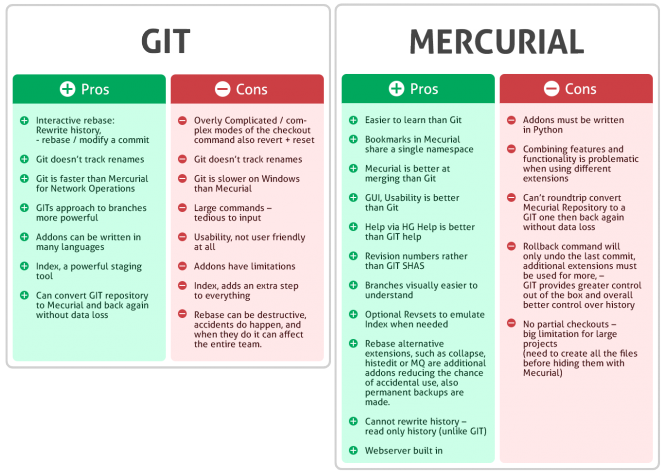
\includegraphics[scale=1]{git-mercurial-pros-cons}
    \caption{Pros y contras de Git y Mercurial\cite{intland_2015:Pros_Cons_Mercurial_Git}}
    \label{fig:git-mercurial-pros-cons}
\end{figure}


\section{Ejercicio 2}
\begin{center}
    \parbox{12cm}{\justify\textit{
        Establece tu nombre de usuario y dirección de correo electrónico. Esto es importante porque las confirmaciones de cambios (commits) en Git usan esta información, y es introducida de manera inmutable en los commits que envías. Utiliza tu usuario y correo de la uco, por ejemplo:}}
    \end{center}


\begin{lstlisting}[xleftmargin=.16\textwidth,language=bash]
$ git config --global user.name "i22lojal"
$ git config --global user.email "i22lojal@uco.es"
\end{lstlisting}

He utilizado los comandos siguientes sin que se produzca ninguna salida por consola.
\begin{lstlisting}[xleftmargin=.16\textwidth,language=bash]
$ git config --global user.name "i12arrae"
$ git config --global user.email "i12arrae@uco.es"
\end{lstlisting}


\section{Ejercicio 3}
\begin{center}
    \parbox{12cm}{\justify\textit{Vamos a crear un nuevo repositorio desde cero (puedes usar uno tuyo o seguir el breve ejemplo que se describe a continuación). Crea en tu cuenta un nuevo directorio que se llame “reposlycs”. Entra en dicho directorio e inicializa el repositorio (\code{\$git init}). Comprueba la creación del directorio .git. ¿Qué función tiene este directorio?
    }}
\end{center}
He creado un directorio en mi home llamado ``prueba''
\begin{lstlisting}[xleftmargin=.16\textwidth,language=bash]
$ cd ~
$ mkdir reposlycs
$ cd reposlycs
$ git init
Inicializado repositorio Git vacío en /home/eduarroyo/reposlycs/.git/
\end{lstlisting}

El comando ha creado un directorio llamado \code{.git}. Este directorio contiene todos los datos que Git necesita para el repositorio local. A destacar:
\begin{itemize}
    \item Directorio objects: contiene todos los objetos del repositorio comprimidos y encriptados.
    \item Archivo config: contiene la configuración de Git para el proyecto
    \item Directorio refs: mantiene las referencias a las direfentes etiquetas y ramas del repositorio.
    \item Archivo HEAD: mantiene una referencia a la rama actual.
\end{itemize}

\section{Ejercicio 4}
\begin{center}
    \parbox{12cm}{\justify\textit{Crea un directorio que cuelgue del anterior llamado ``include''.
    }}
\end{center}
\begin{lstlisting}[xleftmargin=.16\textwidth,language=bash]
$ mkdir include
\end{lstlisting}

\section{Ejercicio 5}
\begin{center}
    \parbox{12cm}{\justify\textit{
        En el directorio ``reposlycs'' escribe un fichero llamado “helloworld.c” que contenga el siguiente código:
    }}
\end{center}

\begin{lstlisting}[style=CStyle,xleftmargin=.3\textwidth]
#include <stdio.h>
int main(void)
{
    printf("Hello World!"); 
}\end{lstlisting}
    
\begin{center}
    \parbox{12cm}{\justify\textit{
        y un fichero ``include/myinclude.h'' que contenga:
    }}
\end{center}

\begin{lstlisting}[style=CStyle,xleftmargin=.3\textwidth]
include <stdio.h>
void f()
{
    printf("Hello World \n");
}\end{lstlisting}

\begin{lstlisting}[xleftmargin=.16\textwidth,language=bash]
$ touch helloworld.c
$ touch include/myinclude.h
\end{lstlisting}

\section{Ejercicio 6}
\begin{center}
    \parbox{12cm}{\justify\textit{
        Añade estos ficheros a tu repositorio y comprueba el estado del repositorio con “git status”. Añade los cambios al stage (\code{\$git add ...}). Haz el primer commit con el mensaje ``Initial commit'' y vuelve a comprobar el estado de tu repositorio.
    }}
\end{center}

Antes de hacer nada, compruebo el estado del repositorio:
\begin{lstlisting}[xleftmargin=.16\textwidth,language=bash]
$ git status
En la rama master

No hay commits todavía

Archivos sin seguimiento:
  (usa "git add <archivo>..." para incluirlo a lo que se será 
  confirmado)

        helloworld.c
        include/

no hay nada agregado al commit pero hay archivos sin seguimiento
presentes (usa "git add" para hacerles seguimiento)
\end{lstlisting}

A continuación añado los dos archivos al seguimiento usando los comandos siguientes:
\begin{lstlisting}[xleftmargin=.16\textwidth,language=bash]
$ git add helloworld.c
$ git add include/myinclude.h
\end{lstlisting}

Hago la primera confirmación de código:
\begin{lstlisting}[xleftmargin=.16\textwidth,language=bash]
$ git commit -m "añadir helloworld.c y myinclude.h"
[master (commit-raíz) 6f325ad] añadir helloworld.c y myinclude.h
 2 files changed, 10 insertions(+)
 create mode 100644 helloworld.c
 create mode 100644 include/myinclude.h
\end{lstlisting}


Vuelvo a comprobar el estado del repositorio:
\begin{lstlisting}[xleftmargin=.16\textwidth,language=bash]
$ git status
En la rama master
nada para hacer commit, el árbol de trabajo está limpio
\end{lstlisting}

\section{Ejercicio 7}
\begin{center}
    \parbox{12cm}{\justify\textit{
        Compila y comprueba lo que ocurre con el ejecutable generado. ¿Se podría añadir el ejecutable al staging y luego al commit?. Haz una prueba. ¿Tendría sentido hacer commit de un ejecutable?
    }}
\end{center}

Compilo:
\begin{lstlisting}[xleftmargin=.16\textwidth,language=bash]
$ gcc helloworld.c -o helloworld
\end{lstlisting}

La compilación ha producido el ejecutable helloworld. Compruebo el estado del repositorio:
\begin{lstlisting}[xleftmargin=.16\textwidth,language=bash]
$ git status
En la rama master
Archivos sin seguimiento:
  (usa "git add <archivo>..." para incluirlo a lo que será
  confirmado)

        helloworld

no hay nada agregado al commit pero hay archivos sin seguimiento
presentes (usa "git add" para hacerles seguimiento)
\end{lstlisting}

Podría agregar el ejecutable al seguimiento con \code{\$ git add helloworld} pero no tiene sentido hacerlo ya que es dependiente del código fuente. Cada desarrollador debe compilar su código local para obtener un ejecutable.
Creo el archivo .gitignore con el contenido helloworld para que git no tenga en cuenta el ejecutable. Añado .gitignore al seguimiento y hago un commit.

\section{Ejercicio 8}
\begin{center}
    \parbox{12cm}{\justify\textit{
        Abre una rama que se llama ``branchA'' y modifica el fichero de la función f() con lo necesario para que f() quede así:
    }}
\begin{lstlisting}[style=CStyle,xleftmargin=.3\textwidth]
void f()
{
    char c1[100]= "Hello world";
    char c2[100]= ", I am <your name here>";
    printf("%s\n", strcat(c1, c2));
    return 0;
}\end{lstlisting}
\end{center}
Creo la rama local ``branchA'':
\begin{lstlisting}[xleftmargin=.16\textwidth,language=bash]
$ git checkout -b branchA
Cambiado a nueva rama 'branchA'
\end{lstlisting}
A continuación realizo la modificación en el archivo en mi editor de texto.

\section{Ejercicio 9}
\begin{center}
    \parbox{12cm}{\justify\textit{
        Realiza el commit con los cambios mencionados en la branchA y el mensaje ``Now with strcat()''.
    }}
\end{center}
\begin{lstlisting}[xleftmargin=.16\textwidth,language=bash]
$git add include/myinclude.h
$ git commit -m "Now with strcat()"
[branchA ed2ee6a] Now with strcat()
 1 file changed, 1 insertion(+)
\end{lstlisting}

\section{Ejercicio 10}
\begin{center}
    \parbox{12cm}{\justify\textit{
        Cambia a la rama master (\code{\$git checkout master}). En la rama master añade un comentario al inicio del fichero ``helloworld.c'' con la fecha y tu nombre como autor del fichero. Realiza el commit de este cambio en la rama master. Con el mensaje ``Now with date and author''
    }}
\end{center}
\begin{lstlisting}[xleftmargin=.16\textwidth,language=bash]
$ git checkout master
Cambiado a rama 'master'
\end{lstlisting}
Modifico el fichero helloworld.c añadiendo un comentario al principio y confirmo el cambio:
\begin{lstlisting}[xleftmargin=.16\textwidth,language=bash]
$ git add helloworld.c
$ git commit -m "Now with date and author"
[master 6bfa915] Now with date and author
 1 file changed, 1 insertion(+)
\end{lstlisting}

\section{Ejercicio 11}
\begin{center}
    \parbox{12cm}{\justify\textit{
        Desde la rama master, fusiona la rama master con la rama branchA. En este caso no hay ningún conflicto, ambas ramas han modificado distintos archivos. Es un merge sin conflicto.
    }}
\end{center}

\begin{lstlisting}[xleftmargin=.16\textwidth,language=bash]
$ git merge branchA
Merge made by the 'recursive' strategy.
 .gitignore           | 1 +
 include/helloworld.h | 5 ++++-
 2 files changed, 5 insertions(+), 1 deletion(-)
 create mode 100644 .gitignore
\end{lstlisting}

\section{Ejercicio 12}
\begin{center}
    \parbox{12cm}{\justify\textit{
        Repite el proceso del punto anterior pero ahora creando un conflicto (merge con conflicto).
    }}
\end{center}
Estando en \code{master}, creo una rama nueva con los comandos
\begin{lstlisting}[xleftmargin=.16\textwidth,language=bash]
$ git branch branchB
eduarroyo@ganimedes:~/reposlycs$ git checkout branchB
Cambiado a rama 'branchB'
\end{lstlisting}
A continuación introduzco una línea en helloworld.c y confirmo los cambios:

\begin{lstlisting}[xleftmargin=.16\textwidth,language=bash]
$ git add helloworld.c 
$ git commit -m "Marca desde BranchB"
[branchB c272698] Marca desde BranchB
    1 file changed, 3 insertions(+), 1 deletion(-)
\end{lstlisting}

Vuelvo a rama master e introduzco un cambio en el helloworld.c y confirmo:
\begin{lstlisting}[xleftmargin=.16\textwidth,language=bash]
$ git checkout master
git checkout master
-- Edito el archivo helloworld.c
$ git add helloworld.c
$ git commit -m "Marca desde master"
[master 8395c14] Marca desde master
 1 file changed, 3 insertions(+), 1 deletion(-)
\end{lstlisting}

Ahora voy a hacer el merge de la rama BranchB:
\begin{lstlisting}[xleftmargin=.16\textwidth,language=bash]
$ git merge BranchB
\end{lstlisting}

\section{Ejercicio 13}
\begin{center}
    \parbox{12cm}{\justify\textit{
        Sube este proyecto a GitHub.
    }}
\end{center}
Primero he creado un repositorio nuevo en mi cuenta de github. Luego he ejecutado el siguiente comando:

\begin{lstlisting}[xleftmargin=.16\textwidth,language=bash]
$ git push --set-upstream https://github.com/eduarroyo/prueba1
.git master
Username for 'https://github.com': eduarroyo
Password for 'https://eduarroyo@github.com': 
Enumerando objetos: 18, listo.
Contando objetos: 100% (18/18), listo.
Compresión delta usando hasta 4 hilos
Comprimiendo objetos: 100% (15/15), listo.
Escribiendo objetos: 100% (18/18), 1.84 KiB | 1.84 MiB/s, listo.
Total 18 (delta 1), reusado 0 (delta 0)
remote: Resolving deltas: 100% (1/1), done.
To https://github.com/eduarroyo/prueba1.git
 * [new branch]      master -> master
Rama 'master' configurada para hacer seguimiento a la rama 
remota 'master' de 'https://github.com/eduarroyo/prueba1.git'.
\end{lstlisting}

\section{Ejercicio 14}
\begin{center}
    \parbox{12cm}{\justify\textit{
        Bájate un proyecto de GitHub de uno de tus compañeros (o de cualquier otra  persona) a tu cuenta local.
    }}
\end{center}

Desde mi home, voy a clonar el repositorio donde tengo las prácticas de la asignatura en \LaTeX :
\begin{lstlisting}[xleftmargin=.16\textwidth,language=bash]
$ cd ~ 
$ git clone https://github.com/eduarroyo/slcs-practicas.git
Clonando en 'slcs-practicas'...
remote: Enumerating objects: 73, done.
remote: Counting objects: 100% (73/73), done.
remote: Compressing objects: 100% (40/40), done.
remote: Total 73 (delta 24), reused 65 (delta 16),
pack-reused 0
Desempaquetando objetos: 100% (73/73), listo.
\end{lstlisting}
Se ha creado el direcotrio slcs-practicas con todo el contenido del repositorio remoto.